\documentclass[a4paper]{article}

%% Language and font encodings
\usepackage[british]{babel}

\usepackage{lmodern}
\usepackage[T1]{fontenc}
\usepackage[utf8x]{inputenc}

%% Sets page size and margins
\usepackage[a4paper, margin=1in]{geometry}

%% Useful packages
\usepackage{tikz}
\usetikzlibrary{arrows,shapes,positioning,shadows,trees}

\usepackage{graphicx}
\usepackage[colorinlistoftodos]{todonotes}
\usepackage[colorlinks=true, allcolors=teal]{hyperref}

\usepackage{fontawesome5}

\usepackage[
backend=biber,
style=apa,
sorting=ynt
]{biblatex}
\addbibresource{biblio.bib}

\title{%
\Large Google Summer of Code 2022 \\
\LARGE Differentiable Rendering}

\author{%
\large Contributor: Leonardo D. Mariscal
\href{mailto:l@mariscal.ch}{\faEnvelope} \href{https://github.com/lmariscal}{\faGithub} \href{https://twitter.com/lmariscal_}{\faTwitter} \href{https://www.linkedin.com/in/leomariscal/}{\faLinkedin} \\
\large Mentors: Dhairya Gandhi, Julian Samaroo \\
\large Project Length: 350hr}

\date{}

\tikzset{
every node/.style={draw,text width=3cm,drop shadow},
style1/.style= {rectangle, rounded corners=3pt, thin,align=center,fill=white!60},
style2/.style= {rectangle, rounded corners=3pt, thin,align=center,fill=white!60},
style3/.style= {rectangle,thin,align=left,fill=white!60}
}

\begin{document}
\maketitle

\section*{Abstract}

% Here should come a list of your milestones. This list is a start based
% on the difference phases of GSoC. Use it as a start. You can/should add
% more details for each phase by breaking it down into weeks or set
% specific targets for each phase. Each target should be split into sub
% task with a time estimate,
% \href{https://en.wikipedia.org/wiki/Work_breakdown_structure}{work
% breakdown structures} are helpful here.

Expand the supported models inside RayTracer.jl by implementing both \textit{Light Field Networks: Neural Scene Representations with Single-Evaluation Rendering} [\cite{NEURIPS2021_a11ce019}], and \textit{Volume Rendering of Neural Implicit Surfaces} [\cite{NEURIPS2021_25e2a30f}].

Port the existing project RayTracer.jl to make use of the latest version of the \textit{FluxML} [\cite{Flux.jl-2018}] libraries. Refactor the automatic differentiation (AD) rules to directly target \textit{ChainRulesCore.jl}.

After finishing the implementation, analyse the performance of the rendering models inside the project, compare them between themselves, and the original implementations.

Identify both the advantages and disadvantages of changing the output format to \textit{OpenEXR}, and changing the internal data representations to use \textit{Flux3D.jl} [\cite{Suthar2020}].

\section*{Introduction}

Rendering is the step of turning a set of data into a 2D image. There have been multiple techniques to achieve this, and the selection of the correct technique heavily depends on the context that the application is based upon.

% In real time graphics, rasterization has been the technique of choice, since it allows us to send vertices to the GPU via graphics APIs, together with information on how to properly paint and connect these vertices to quickly form a mesh. This approach takes advantage of the parallelizable nature that painting pixels via the same algorithm from already defined data has. \\
An approach that is mostly used in offline rendering
%, but has as of late made its appearance in real time graphics due to the advancements in hardware,
is ray tracing. It allows us to simulate how real light would behave, and approximate how we would see certain materials in certain parameters. Defining these materials, and parameters is both time and resource heavy, since it is necessary to add all the information that the rendering function requires to accurately simulate how light would react.

If we have a sample 2D image of the output scene that we want to simulate, we can approach this issue as a machine learning inverse problem. Using the 2D image, we can use differentiable rendering and an appropriate model to train a neural network (NN) to infer both the material and scene information that we need.

\textit{RayTracer.jl} [\cite{Pal2020}] capitalizes on the Julia architecture, and ecosystem to create a differentiable ray tracer which is able to directly infer the scene parameters to recreate the image that was used as an input. It makes use of Zygote [\cite{Zygote.jl-2018}] to seamlessly differentiate the rendering function, via source-to-source automatic differentiation (AD), and with no changes to the renderer itself to make it differentiable. With this gradient, it also uses the \textit{FluxML} [\cite{Flux.jl-2018}] framework to create a NN and be able to solve rendering tasks pertaining to inverse graphics problems.

We want to expand upon this solid base of components and differentiable pipeline to handle other rendering models. These other models approach the inferring process from a novel perspective, and handle both the geometry and the 3D neural scene representation differently. \textit{LFN} [\cite{NEURIPS2021_a11ce019}] makes use of meta-learning to construct a consistent scene representation using as little as a single image observation, while using only a single network evaluation per ray. \textit{VolSDF} [\cite{NEURIPS2021_25e2a30f}] changes the approach to neural volume rendering, by modelling the volume density as a transformed version of the learned surface geometry, instead of the geometry being a function of the volume density. This allows to bound the opacity approximation error leading to higher fidelity in the sampling.

\section*{Technical Details}

% Long description of the project. \textbf{Must} include all technical
% details of the projects like libraries involved.

% Here it is important to show if you had previous conversations with your
% mentors. You can show relevant pieces of code that you want to change.
% You can link to literature you used during the research.

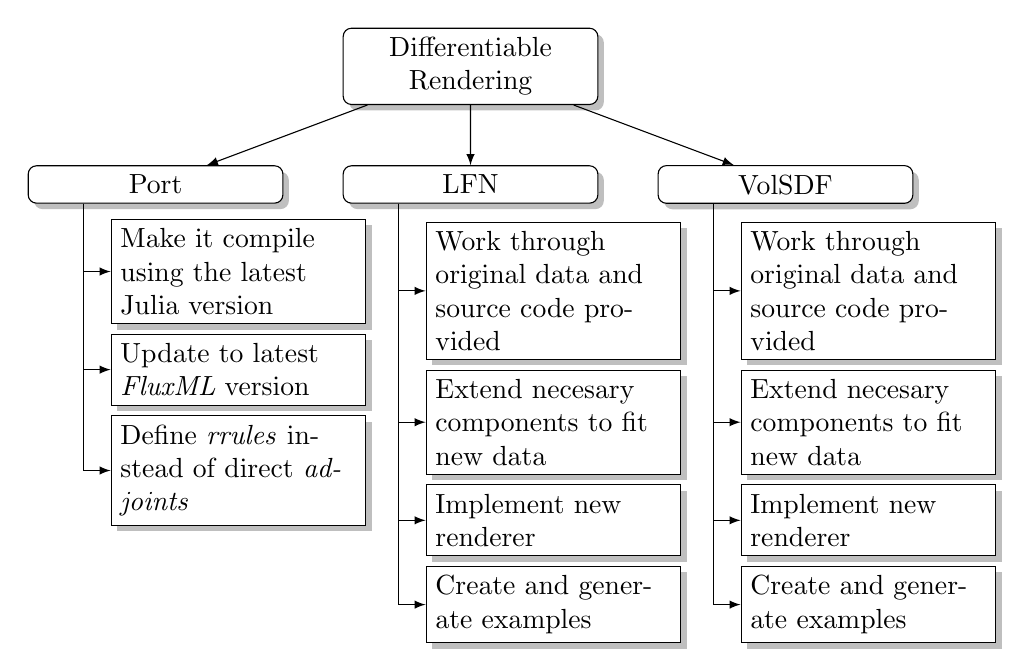
\begin{tikzpicture}[
remember picture,
level 1/.style={sibling distance=40mm},
edge from parent/.style={->,draw},
>=latex]

\node[style1] {Differentiable Rendering}
child {node[style2] (c1) {Port}}
child {node[style2] (c2) {LFN}}
child {node[style2] (c3) {VolSDF}};

\node [style3,below of = c1,xshift=30pt,yshift=-3pt] (c11) {Make it compile using the latest Julia version};
\node [style3,below of = c11,yshift=-7pt] (c12) {Update to latest \textit{FluxML} version};
\node [style3,below of = c12,yshift=-8pt] (c13) {Define \textit{rrules} instead of direct \textit{adjoints}};

\node [style3,below of = c2,xshift=30pt,yshift=-10pt] (c21) {Work through original data and source code provided};
\node [style3,below of = c21,yshift=-19pt] (c22) {Extend necesary components to fit new data};
\node [style3,below of = c22,yshift=-7pt] (c23) {Implement new renderer};
\node [style3,below of = c23,yshift=-2pt] (c24) {Create and generate examples};

\node [style3,below of = c3,xshift=30pt,yshift=-10pt] (c31) {Work through original data and source code provided};
\node [style3,below of = c31,yshift=-19pt] (c32) {Extend necesary components to fit new data};
\node [style3,below of = c32,yshift=-7pt] (c33) {Implement new renderer};
\node [style3,below of = c33,yshift=-2pt] (c34) {Create and generate examples};

\foreach \value in {1,...,3}
  \draw[->] (c1.195) |- (c1\value.west);

\foreach \value in {1,...,4}
  \draw[->] (c2.195) |- (c2\value.west);

\foreach \value in {1,...,4}
  \draw[->] (c3.195) |- (c3\value.west);
\end{tikzpicture}

\section*{Schedule of Deliverables}

\subsection*{19 April -- 13 June}

Familiarize myself with the Julia ML ecosystem. Translating my previous experience in Python to the active packages that will be used inside the project. These packages would include, \textit{Flux3D}, the \textit{FluxML} framework, \textit{ChainRules.jl} together with \textit{ChainRulesCore.jl}, \textit{Zygote}, and \textit{OpenEXR} among other utility packages.

Establish the repository that will be used. Together with setting up a Git workflow.

Get to know mentors, keep up with ML packages developed, and integrate myself with the community by attending events like \textit{ML Community + FastAI.jl Dev Call}.

Continue reading literature on the topic, by working through the original implementations and recreating results of the published research.

Set up a blog, in order to comply with the blog posts requirement. This blog will be hosted under\\
\url{https://mariscal.ch/}

\subsection*{13 June -- 1 July}

Port the existing codebase to the latest version of Julia and the \textit{FluxML} framework. Identify what changes can be done to better make use of any features released in between.

Analyse if using \textit{OpenEXR} as the output format benefits the project as a whole. Together with analysing if using \textit{Flux3D} as the internal 3D data representation outperforms the existing solution, and if it does what changes need to be done to the existing codebase. 

Abstract the existing components for them to handle the data required for the new rendering models. Together with abstracting how the optimization, gradients, and the scene representation is managed internally.

\pagebreak

\subsection*{1 July -- 29 July}

Work through the data provided by the original authors, and transform it to something we can work with.

Implement the \textit{LFN} rendering model by going th through the original implementation and identifying key features that need to be added to the existing solution, in the components, scene representation, and how the output is managed.

Add necessary adjoints in \textit{Zygote} by creating the required \textit{rrules} using \textit{ChainRulesCore.jl}

Making use of the AD function, create a NN using \textit{Flux} to manage the optimization for the inputs given.

Create examples on the renderer model, and tests to verify implementation.

\subsection*{29 July -- 5 September}

Work through the data provided by the original authors, and transform it to something we can work with.

Implement the \textit{VolSDF} rendering model by going through the original implementation and identifying key features that need to be added to the existing solution, in the components, scene representation, and how the output is managed.

Add necessary adjoints in \textit{Zygote} by creating the required \textit{rrules} using \textit{ChainRulesCore.jl}

Making use of the AD function, create a NN using \textit{Flux} to manage the optimization for the inputs given.

Create examples on the renderer model, and tests to verify implementation.

\subsection*{5 September -- 12 September}

Analyse the performance of the implemented models, between themselves, and compared to the original implementations, \textit{LFN} in \textit{C++}, and \textit{VolSDF} using \textit{Python}. Create figures using \textit{Makie} or a similar package to present in the bi-weekly reports. \\

LFN \url{https://www.vincentsitzmann.com/lfns/} \href{https://github.com/vsitzmann/light-field-networks}{Repo} \href{https://drive.google.com/drive/folders/15u6WD0zSBXzu8jZBF-Sn5n01F2HSxFCp}{Data}

VolSDF \url{https://lioryariv.github.io/volsdf/} \href{https://github.com/lioryariv/volsdf}{Repo} \href{https://www.dropbox.com/sh/oum8dyo19jqdkwu/AAAxpIifYjjotz_fIRBj1Fyla}{Data}

% \subsection*{Community Bonding Period}

% This phase is to get to know the community better. Check that your build
% environment is setup. This time should also be used to discuss your
% project in more detail with the community and in general introduce it.

% \emph{Note:} We require you to write regular blog posts. Now is a good
% time to make sure your blog works and send us the link.

% Set up a blog, in order to comply with the blog posts requirement. It will be hosted under\\ \url{https://mariscal.ch/}.

% Attend \textit{ML Community + FastAI.jl Dev Call}, previously called \textit{ML and AD Development/Usage Call}s which are hosted every two weeks via zoom, in order to keep up with development and interact with the community.

% \subsection*{Phase 1}

% % At the end of Phase 1, \textit{RayTracer.jl} would have already been ported, and the rules written using \textit{ChainRulesCore.jl}. \textit{LFN} implementation should be in development, 
% Port \textit{RayTracer.jl} to the latest version of Julia, and update all the libraries used. Update all the \textit{adjoints} to make use of \textit{ChainRulesCore.jl}. Identify if \textit{OpenEXR} would be a better format to set as the output; together with testing if using \textit{Flux3D.jl} [\cite{Suthar2020}] to represent the data in some components is adequate. Start with the implementation of \textit{LFN}.

% \subsection*{Phase 2}

% Finish implementation of both new renderer models, \textit{LFN}, and \textit{VolSDF}. Start by reproducing their results, making use of the provided source-code and their data used, \textit{C++}, and \textit{Python} respectively. Identify how the existing components need to be updated to support all the necessary data. Implement the rendering models, and extend any required \textit{rrules}.

% \subsection*{Final Week}

% % At this stage you should finish up your project. At this stage you
% % should make sure that you have code submitted to your organization. Our
% % criteria to mark your project as a success is to submit code before the
% % end of GSoC.
% Create examples of both render models which would also work as tests of the implementation. Compare all the rendering models, graph performance of all the examples, and if possible, of the original source provided in the papers.

\section*{Deliverables}

\begin{itemize}
    \item \textbf{Phase 1} - \textit{RayTracer.jl} using the latest \textit{FluxML} libraries, with its automatic differentiation extended rules setup using \textit{ChainRulesCore.jl}. If appropriate, have the output format implemented as OpenEXR, and change the internal data representation to use \textit{Flux3D}. 
    
    \item \textbf{Phase 2} - Implementation of both of the suggested rendering models, \textit{LFN} and \textit{VolSDF}, by expanding the components to handle the necessary data, implementing the required rendering functions, configuring any required \textit{rrules} for AD, and creating the required NN using \textit{Flux}.
    
    \item \textbf{Across the phases} - Analysis of the implemented renderers inside the project, compared to themselves, and to the original implementations. These analyses would be in form of graphs, and conclusions based on those results, both would be included in the bi-weekly blogs.
\end{itemize}

\pagebreak

\section*{Development Experience}

% Do you have code on github? Can you show previous contributions to other
% projects? Did you do other code related projects or university courses?
My GitHub profile is \url{https://github.com/lmariscal}. I have ample experience in real-time rendering, mostly related to games and interactive computer graphics. This while also keeping up to date with neural scene representation research. Deeply in love with converting data into beautiful 2D images.

As for Julia specifically, I have mostly used it for competitive programming challenges, like AdventOfCode. This would be my first big project using this language. Currently using Arch Linux, and feel comfortable using the Julia ecosystem, including the LSP, the package manager, the documentation system, making use of the REPL and its debug features, and in use of the language in general. My main area of focus in the Community phase would be to familiarize myself with the Machine Learning, and Automatic Differentiation libraries the Julia ecosystem has, and that I will be using inside the project. Having made use of both \textit{PyTorch}, and \textit{JAX} in the past, it would mean translating that experience to the Julia ecosystem.

% \section*{Other Experiences}

\section*{Why this project?}

% Why you want to do this project?
My interest in differential rendering started with the publication of \textit{Neural Radiance Fields} [\cite{mildenhall2020nerf}], its ability to generate novel views truly blew my mind. Since then, I have kept up with the literature by attending computer vision, and computer graphics conferences---thankfully they have been virtual these past few years---while also reading journals, and keeping up to date on Arxiv. It took me a while to specifically select these two papers to implement, but they are the ones that most caught my attention, and both of them come with fully open-sourced implementations and the data used.

Julia has been one of the languages that was in my radar, but have had no particular project to implement in the language. I feel that this project is perfect to jump into, as it already has a solid base, and it has the promise of demonstrating that Julia is productive and efficient for implementing these kinds of models, while showcasing all of its strengths and its ecosystem. The plan after GSoC is to make use of this project for my Master's thesis, which would itself expand from the work of \textit{LFN} [\cite{NEURIPS2021_a11ce019}].

% \section*{Appendix}

% Extra content

\printbibliography

\end{document}